\section{Phenix Real Space Refine protocol}
\label{app:realSpaceRefineProtocol}%a140
Protocol designed to refine in real space an atomic structure into a map in \scipion by using \iii{phenix.real\_space\_refine} program \citep{afonine2018}. Integrated in the $Phenix$ software suite (\url{https://www.phenix-online.org/}), \iii{phenix.real\_space\_refine} tool can be applied to refine models generated both from cryo-EM and from crystallography. This program computes \ttt{Real Space Correlation} coefficients between map and model-derived map and, additionally, it assesses the geometry and dihedral-angle combinations of atomic structures with the aim of getting the best map-fitted structure by reducing the number of geometry outliers.   Validation $MolProbity$ scores are shown at the end of the refinement process.

\begin{itemize}
 \item Requirements to run this protocol and visualize results:
    \begin{itemize}
        \item \scipion plugin: \ttt{scipion-em-phenix}
        \item PHENIX software suite (version 1.13-2998)
        \item \scipion plugin: \ttt{scipion-em-chimera}
    \end{itemize}
 \item \scipion menu:\\
  \ttt{Protocols SPA -> Model building} (\ffigure{fig:app_protocol_real_space_refine_1} (A))
  
 \item Protocol form parameters (\ffigure{fig:app_protocol_real_space_refine_1} (B)):
  
    \begin{figure}[H]
     \centering 
     \captionsetup{width=.7\linewidth} 
     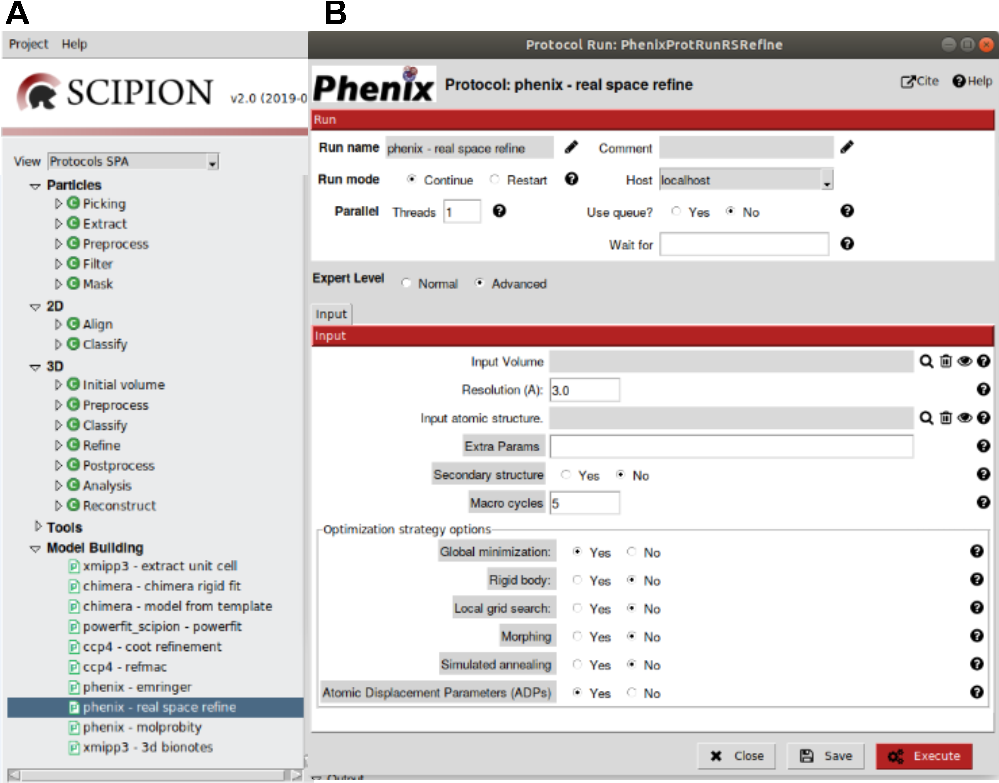
\includegraphics[width=0.90\textwidth]{Images_appendix/Fig148.pdf}
     \caption{Protocol \scommand{phenix - real space refine}. A: Protocol location in \scipion menu. B: Protocol form.}
     \label{fig:app_protocol_real_space_refine_1}
    \end{figure}
    
    \begin{itemize}
     \item \ttt{Input Volume}: Electron density map previously downloaded or generated in \scipion.
     \item \ttt{Resolution (\AA)}: \ttt{Input Volume} resolution.
     \item \ttt{Input atomic structure}: Atomic structure previously downloaded or generated in \scipion and fitted to the electron density map.
     \item \ttt{Extra Params}: Advanced param that allows to add a string to the phenix command including other \iii{phenix.real\_space\_refine} program params. Syntax to add extra params: \ttt{paramName1} = \ttt{value1} \ttt{paramName2} = \ttt{value2}
     \item \ttt{Secondary structure}: Advanced param to choose including secondary structure restraints. It is set to \ttt{No} by default.
     \item \ttt{Macro cycles}: Advanced param that allows select the number of iterations of refinement. Although 5 macro-cycles, set by default, is usually enough, increasing this value might be helpful when model geometry or/and model-to-map fit is poor. Increment the number of macro-cycles will also scale the computing times.
     \item \ttt{Optimization strategy options}: Box of advanced params that allow modify the default refinement optimization strategy:
      \begin{itemize}
       \item \ttt{Global minimization}: Param set to ``Yes'' by default to look for the global minimum of the model. 
       \item \ttt{Rigid body}: Param set to ``No'' by default. It considers the movement of groups of atoms as a single body.
       \item \ttt{Local grid search}: Param set to ``No'' by default. It is used to fit local rotamers.
       \item \ttt{Morphing}: Param set to ``No'' by default. It allows distortions of the model to match the electron density map.
       \item \ttt{Simulated annealing}: Param set to ``No'' by default. By molecular dynamics this param minimizes the energy of the model.
       \item \ttt{Atomic Displacement Parameters (ADPs)}: Param set to ``Yes'' by default. Model refinement regarding the map param that considers temperature factors. This refinement step is performed only at the last macro-cycle.
      \end{itemize}
    \end{itemize}
 
 \item Protocol execution:\\
 Adding specific map/structure label is recommended in \ttt{Run name} section, at the form top. To add the label, open the protocol form, press the pencil symbol at the right side of \ttt{Run name} box, complete the label in the new opened window, press OK and, finally, close the protocol. This label will be shown in the output summary content (see below). If you want to run again this protocol, do not forget to set to \ttt{Restart} the \ttt{Run mode}.\\
  Press the \ttt{Execute} red button at the form bottom.
  
 \item Visualization of protocol results:
 
 After executing the protocol, press \ttt{Analyze Results} and the results window will be opened (\ffigure{fig:app_protocol_real_space_refine_2}). 
  
    \begin{figure}[H]
     \centering 
     \captionsetup{width=.7\linewidth} 
     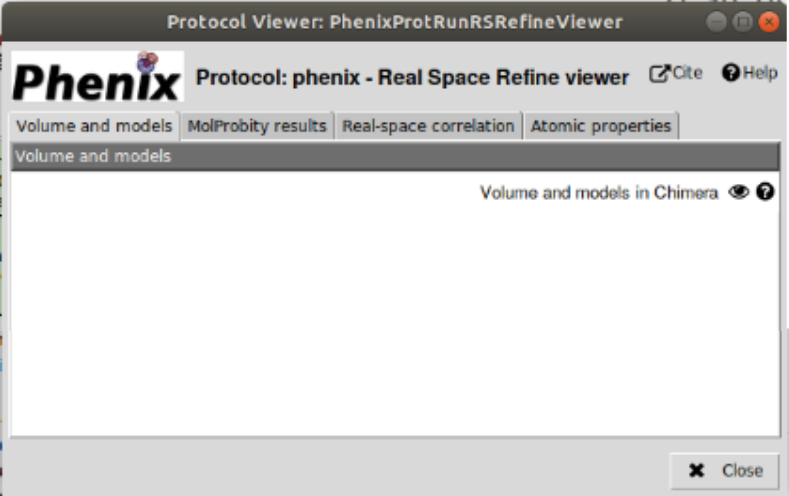
\includegraphics[width=0.60\textwidth]{Images_appendix/Fig149.pdf}
     \caption{Protocol \scommand{phenix - real space refine}. Taps to visualize $MolProbity$  and \iii{Real Space Refine} correlation results.}
     \label{fig:app_protocol_real_space_refine_2}
    \end{figure}
    
Four taps are shown in the upper part of the results window:
   \begin{itemize}
     \item \ttt{Volume and models}: \chimera graphics window will be opened by default. Atomic structure and volume are referred to the origin of coordinates in \chimera. To show the relative position of atomic structure and electron density volume, the three coordinate axes are represented; X axis (red), Y axis (yellow), and Z axis (blue) (\ffigure{fig:app_protocol_volume_3}).
     \item \ttt{MolProbity results} (\ffigure{fig:app_protocol_real_space_refine_3}):
        \begin{figure}[H]
         \centering 
         \captionsetup{width=.7\linewidth} 
         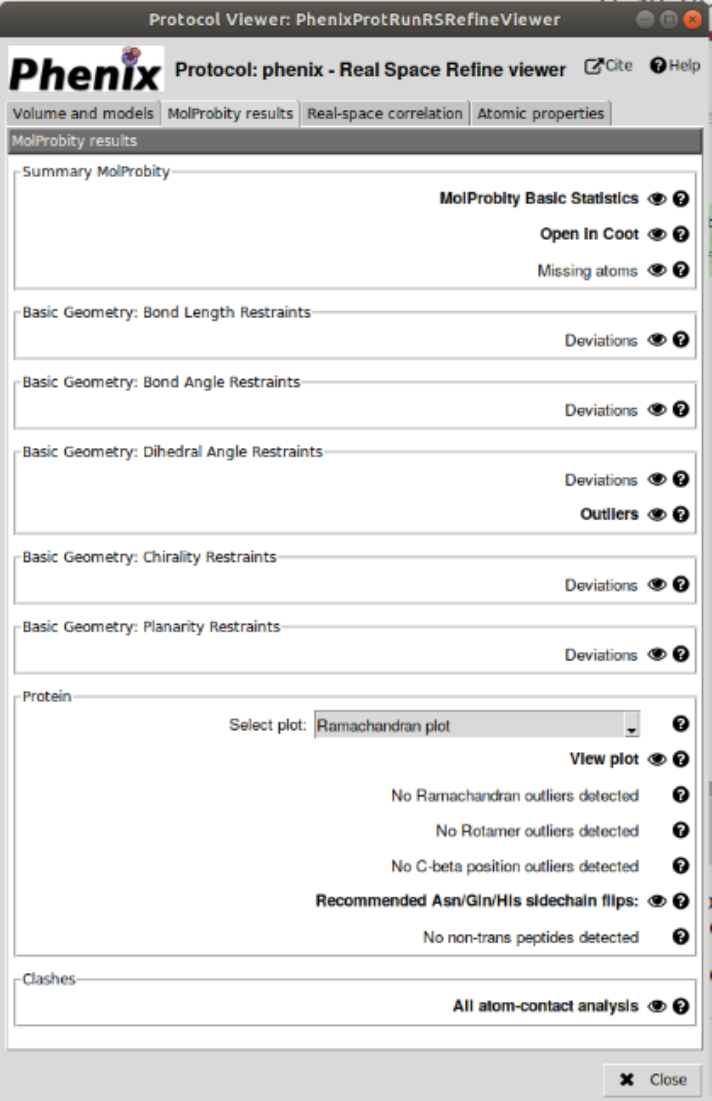
\includegraphics[width=0.65\textwidth]{Images_appendix/Fig150.pdf}
         \caption{Protocol \scommand{phenix - real space refine}. \phenix \ttt{real space refine} results.}
         \label{fig:app_protocol_real_space_refine_3}
        \end{figure}
        
        \begin{itemize}
         \item \ttt{Summary MolProbity}: 
          \begin{itemize}
           \item \ttt{MolProbity Basic Statistics}: Statistics computed by the $Phenix$ package to assess protein geometry using the same distributions as the MolProbity server:\setlength{\parindent}{12pt}
           
            \ttt{Ramachandran outliers}: Percentage of residues assessed that show an unusual combination of their $\phi$ (C-N-CA-C) and $\psi$ (N-CA-C-N) dihedral angles.
            
            \ttt{Ramachandran favored}: Percentage of residues assessed that show an normal combination of their $\phi$ (C-N-CA-C) and $\psi$ (N-CA-C-N) dihedral angles. Ramachandran outliers and favored residues are detailed in the \ttt{Ramachandran plot}, shown below. Allowed residues are included in the small region comprised between favored and outlier regions of that plot.
            
            \ttt{Rotamer outliers}: Percentage of residues assessed that adopt an unusual conformation of $\chi$ dihedral angles. Rotamer outliers, commonly used to characterize the conformation of protein sidechains, are detailed in Chi1-Chi2 plot, shown below.
            
            \ttt{C-beta outliers}: Number of residues showing an unusual deviation (higher than 0.25 \AA) of the C{$\beta$} from its ideal position. This deviation is an indicator of incompatibility between sidechain and backbone. 
            
            \ttt{Clahscore}: Score associated to the number of pairs of non-bonded atoms unsually close to each other, showing probable steric overlaps. Clashscore is calculated as the number of serious clashes per 1000 atoms. This value has to be as low as possible.
            
            \ttt{RMS (bonds)}: Root-mean-square deviation of molecule bond lengths.
            
            \ttt{RMS (angles)}: Root-mean-square deviation of molecule bond angles.
            
            \ttt{Overall score}: $MolProbity$ overall score representing the experimental resolution expected for the structure model. This value should be lower than the actual resolution. The lower the value, the better quality of the structure model.
           
           \item \ttt{Open in Coot}: Interactive visualization and structure modification tool for Ramachandran, Rotamer and C{$\beta$} outliers, as well as severe clashes. Coot graphics window will be centered on the specific atom or residue outlier when it is clicked.
           
           \item \ttt{Missing atoms}: For clarity, hydrogen atoms are not included.
          \end{itemize}
          
         \item \ttt{Basic Geometry: Bond Length Restraints}: Bonded pairs of atoms outliers according to the bond restraints between pairs of bonded atoms. The \ttt{Deviations} table indicates the number of outliers and the number of restraints (in accordance with the geometry restraints library). Those outliers appear sorted by deviation (higher than 4 sigmas) in the \ttt{Outliers} list.
         \item \ttt{Basic Geometry: Bond Angle Restraints}: Bonded triplets of atoms outliers according to the angle restraints between triplets of bonded atoms. The \ttt{Deviations} table indicates the number of outliers and the number of restraints (in accordance with the geometry restraints library). Those outliers appear sorted by deviation (higher than 4 sigmas) in the \ttt{Outliers} list.
         \item \ttt{Basic Geometry: Dihedral Angle Restraints}: Bonded tetrads of atoms outliers according to the dihedral angle restraints between tetrads of bonded atoms. The \ttt{Deviations} table indicates the number of outliers and the number of restraints (in accordance with the geometry restraints library). Those outliers appear sorted by deviation (higher than 4 sigmas) in the \ttt{Outliers} list.
         \item \ttt{Basic Geometry: Chilarity Restraints}: Bonded tetrads of atoms outliers according to the chilarity restraints between tetrads of bonded atoms. The \ttt{Deviations} table indicates the number of outliers and the number of restraints (in accordance with the geometry restraints library). Those outliers appear sorted by deviation (higher than 4 sigmas) in the \ttt{Outliers} list.
         \item \ttt{Basic Geometry: Planarity Restraints}: Bonded groups of atoms outliers according to the planarity restraints between groups of bonded atoms. The \ttt{Deviations} table indicates the number of outliers and the number of restraints (in accordance with the geometry restraints library). Those outliers appear sorted by deviation (higher than 4 sigmas) in the \ttt{Outliers} list.
         \item \ttt{Protein}: Box validating protein geometry:
         \begin{itemize}
          \item \ttt{Select plot}: Box to select a plot to visualize: The Ramachandran plot or the Chi1-Chi2 plot.
          \item \ttt{View plot}: Visualization of the plot previously selected.
          \item \ttt{Ramachandran outliers}: List of Ramachandran residue outliers with their respective $\phi$ (C-N-CA-C) and $\psi$ (N-CA-C-N) dihedral angle values.
          \item \ttt{Rotamer outliers}: List of Rotamer residue outliers with their respective $\chi$ dihedral angles.
          \item \ttt{C-beta outliers}: List of C{$\beta$} residue outliers with their respective angles (angular position of \ttt{C-beta} atom in radial space).
          \item \ttt{Recommended Asn/Gln/His sidechain flips}: Asn, Gln and His residues, harboring asymmetric sidechains, recommended to be flipped to form favourable van der Waals contacts and hydrogen bonds.
          \item \ttt{Cis and Twisted peptides}: Residues showing $cis$ or $twisted$ conformations that could be modeling errors.
         \end{itemize}

         \item \ttt{Clashes}: Box to detail \ttt{All atom-contact analysis}, the list that contains all severe clashes (non-H atoms overlaping more than 0.4 \AA) and that can be checked in \coot.
        \end{itemize}
      \item \ttt{Real-space correlation} (\ffigure{fig:app_protocol_real_space_refine_4}):
       \begin{figure}[H]
         \centering 
         \captionsetup{width=.7\linewidth} 
         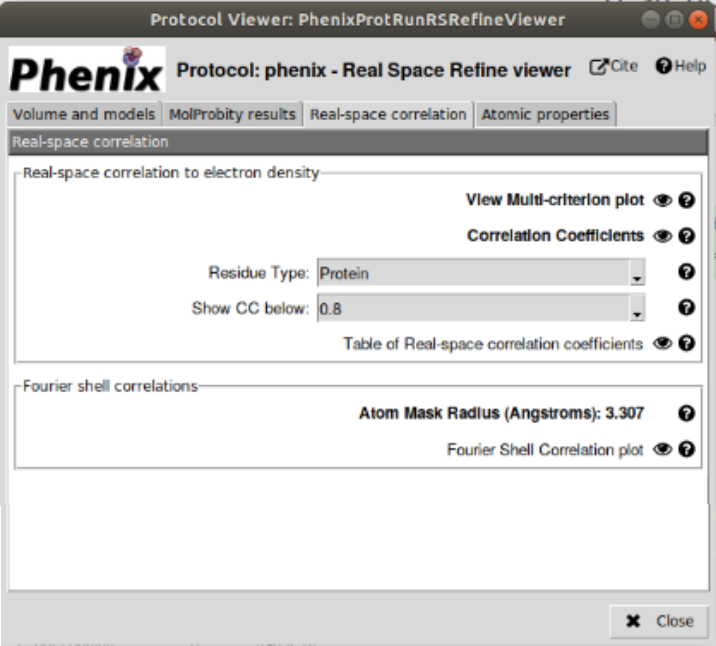
\includegraphics[width=0.65\textwidth]{Images_appendix/Fig151.pdf}
         \caption{Protocol \scommand{phenix - real space refine}. Real-space correlation results.}
         \label{fig:app_protocol_real_space_refine_4}
        \end{figure}
        \begin{itemize}
         \item \ttt{Real-space correlation to electron density}: 
         \begin{itemize}
          \item \ttt{View Multi-criterion plot}: Plot showing cross-correlation and B-factor values for each residue of the macromolecule over 100-residue regions. Additional validation information, such as Ramachandran, Rotamer or C{$\beta$} outliers, is also detailed, as well as severe clashes.  
          \item \ttt{Correlations Coefficients}: Three Real-space correlation coefficients are computed \citep{afonine2018b}: \setlength{\parindent}{12pt}
          
           \ttt{Mask CC}: Correlation coefficient between experimental volume and model-derived map inside the mask region around the model.
           
           \ttt{Volume CC}: Correlation coefficient that considers only map regions with the highest density values, ignoring regions below a certain contouring density threshold. Particularly, in this case the N points with the highest density, inside the molecular mask, are taken into account.
           
           \ttt{Peak CC}: Correlation coefficient that considers only map regions with the highest density values, ignoring regions below a certain contouring density threshold. Particularly, in this case the N points with the highest density, simultaneously present in the model-calculated map and in the experimental map, are taken into account.

          \item \ttt{Residue Type}: Box to select a type of residue: protein residue, other (for example heteroatom), water or everything. Protein residue is selected by default.
          \item \ttt{Show CC below}: Box to select the maximum limiting value of correlation coefficient shown by the residue type selected. 
          \item \ttt{Table of Real-space correlation coefficients}: List displaying the selected residues with correlation coefficient value lower than the maximum value selected above. Residues showing the lower correlation might indicate errors in modeling of specific regions of the model.
         \end{itemize}
         
         \item \ttt{Fourier shell correlations}:
          \begin{itemize}
           \item \ttt{Atom Mask Radius (Angstroms)}: Radius of the ``Fourier Shell'', a spherical volume mask in Fourier space.
           \item \ttt{Fourier Shell Correlation plot}: FSC plot regarding the inverse of the spatial frequency.
          \end{itemize}
        \end{itemize}
      \item \ttt{Atomic properties} (\ffigure{fig:app_protocol_molprobity_5}): Atom numerical properties:
       \begin{figure}[H]
         \centering 
         \captionsetup{width=.7\linewidth} 
         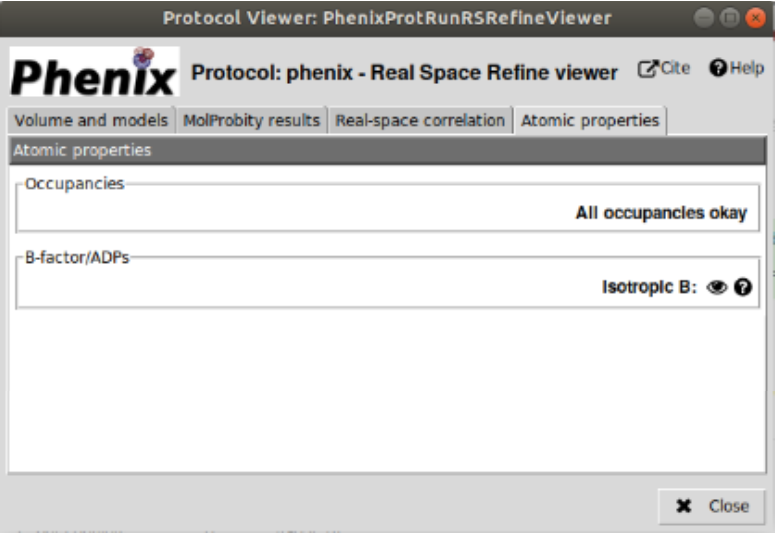
\includegraphics[width=0.65\textwidth]{Images_appendix/Fig152.pdf}
         \caption{Protocol \scommand{phenix - real space refine}. Atomic properties results.}
         \label{fig:app_protocol_real_space_refine_5}
        \end{figure}
        \begin{itemize}
         \item \ttt{Occupancies}: Atomic property used in crystallography. It represents the fraction of molecules in which a specific atom is in a given position or conformation at any given time. The sum of occupancies has to be 1 in total. Occupancies of zero indicate that no experimental data support the position of the atom in the model.
         \item \ttt{B-factor/ADPs}: Temperature factors reflect the vibration status of the atoms in which the observed electron density constitutes an average of all the small motions. Low values (around 10) indicate low vibration of atoms, whereas high values (around 50) show atoms moving so much that locate them properly results difficult. This last is usually the case of atoms located at the protein surface.
          \begin{itemize}
           \item \ttt{Isotropic B}: Temperature factor constrained to be the same in all three directions. By clicking here, a table showing the statistics (\ttt{Min}, \ttt{Max} and \ttt{Mean}) of the isotropic B-factor is displayed.
          \end{itemize}
        \end{itemize}
    \end{itemize}
    
 \item Summary content:
 
  \ttt{SUMMARY} box:\\Main statistics included in the above $MolProbity$ \ttt{Model Final Statistics} table.

\end{itemize}
